
\chapter{Position of the Project}
\label{chap:project}


\section{Recapitulation and forecast}

This project is designed to automate a sniffer to detect attack. The most important fact is that our sensors need
to detect a strategy of attack and not only patterns of attack. After our bibliographic studies, it is simple to
understand that we will use an IDS with an anomaly detection method. We will use SELKS\footnote{A description of
  SELKS is available page \pageref{chap:selks}} because it is the main free open source IDS available on the
market. A description of our technical choice is explained in the next section.

As suggested in the description of the project delivered by our professor, we also use Hynesim to automate tests
and simulate our solutions. In this way, we will have the ability to justify the effectiveness of our solution.
To do that we will run many possible attack scenarios.

\section{Technical choice}

We will firstly achieve a network infrastructure on Hynesim. We will install a basic infrastructure with only one
server. Then, we will put on our network, a SLEKS server as a simple IDS which we will configure. We choose, to
implement firstly a pattern matching method. We will also put an attacker on the network and we will achieve simple
attacks to test our infrastructure. It is possible to see the infrastructure in the figure \ref{fig:network_hynesim}.

\begin{figure}[h]
  \centering
  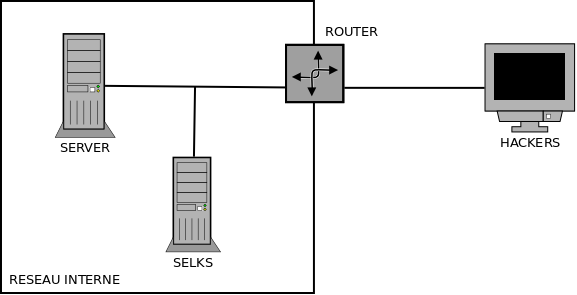
\includegraphics[width=0.7\textwidth]{reseau_hynesim}
  \caption{Hynesim network architecture}
  \label{fig:network_hynesim}
\end{figure}

After this installation, we will try to improve the system. We will implement an anomaly detection method. In this
way, the IDS will have the ability to detect a will to attack. One of the most important difficulties will be to
not raise alert for normal utilization.

\section{Forecasting organization}

\subsection{Kanban}

To achieve this project, we decided to use some tools to arrange our work. First of all, we decided to use an agile
technique of management which name Kanban.~\\

\definition{Kanban}{Kanban is a new technique for managing a software development process in a highly efficient
  way. Kanban underpins Toyota's "just-in-time" (JIT) production system. The kanban system consists of a big board on
  the wall with cards or sticky notes placed in columns with numbers at the top \cite{peterson:kanban}}


Kanban is an inventory-control system to control the supply chain. It uses a board with columns. Each column
represents a status, for example: to do, doing, done. In each column we put <<notes>> which represent a task.
Moreover, each column has a maximum number of notes authorized.


\begin{figure}[h]
  \centering
  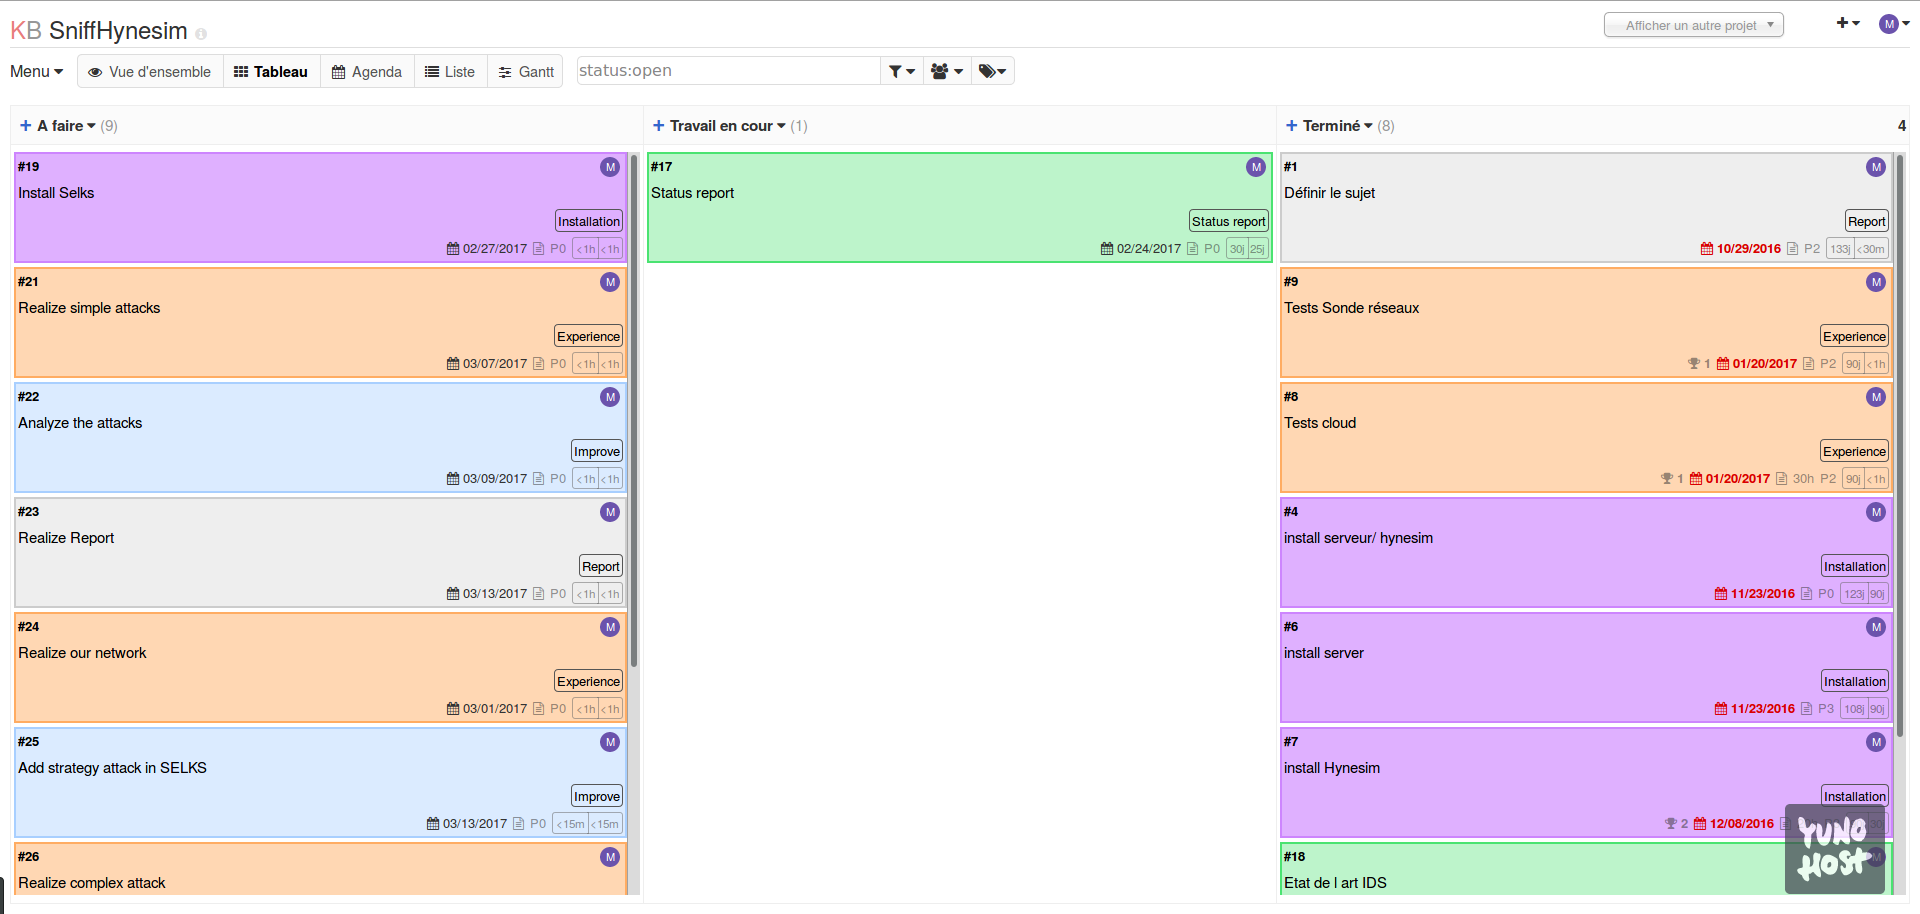
\includegraphics[width=\textwidth]{kandboard}
  \caption{Kanboard of this project}
  \label{fig:kanboard}
\end{figure}


Limiting the amount of tasks, at each step in the process, prevents overproduction and reveals bottlenecks
dynamically. In fact, with this technique it is possible to have a better overview of the project and control it
dynamically.
~\\

For this project, we use Kanboard\cite{guillot:kanboard} self-hosted on our own Yunohost server.\footnote{ It is possible to
  see our kanboard at this link:
  \url{https://mic-rigaud.fr/kanboard/?controller=BoardViewController&action=readonly&token=10ea65eca908023dbcd8bc8dce75791c7a14d67912627dafaa5b71033222}}.
You can see in the figure \ref{fig:kanboard} the kanboard of this project. Each color represent a category of tasks:
blue: improvement , purple: installation, red : experience, green: status report, and grey: report.

With this tool, it is also possible to see tasks as a Gantt diagram. The figure \ref{fig:grantt} presents our
Gantt diagram.

\begin{figure}[h]
  \centering
  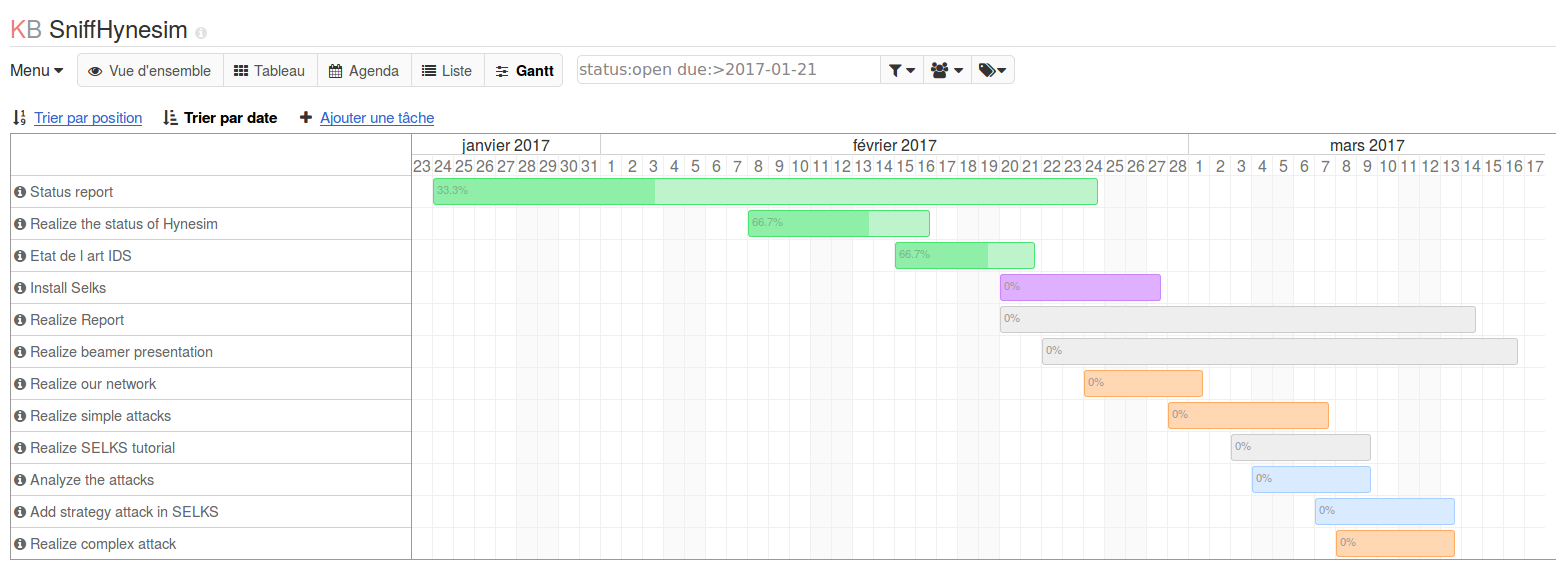
\includegraphics[width=\textwidth]{grant}
  \caption{Gantt diagram of the project}
  \label{fig:grantt}
\end{figure}


\subsection{Github}

To achieve this project, we also decided to use Git and Github as a Git server. ~\\

\definition{Git}{Git is a version control system for tracking changes in computer files and coordinating work on
  those files among multiple people.}

Git enables me to control version of our work and obtain a real showcase of it for our tutor. The figure
\ref{fig:github} is a screenshot of our Github server.

\begin{figure}[h]
  \centering
  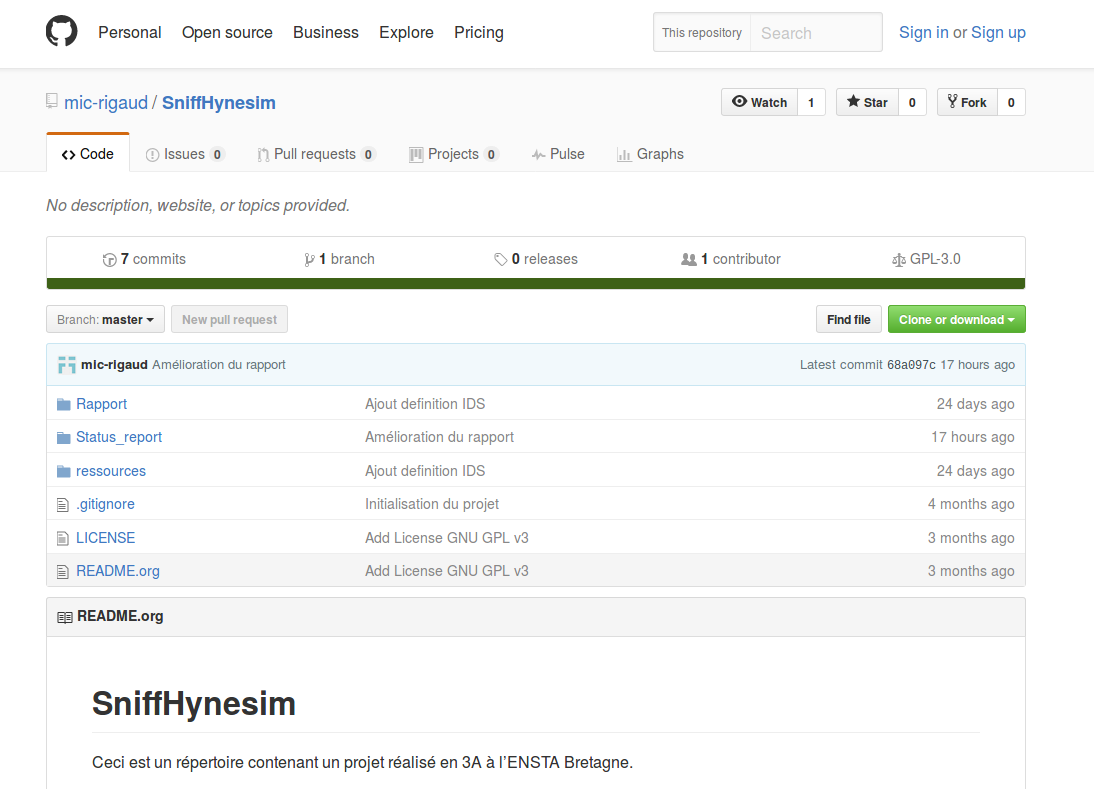
\includegraphics[width=\textwidth]{github}
  \caption{Github server}
  \label{fig:github}
\end{figure}




%%% Local Variables:
%%% mode: latex
%%% TeX-master: "../rapport_de_base"
%%% End:
